\chapter{Experiments}
\label{experiments_chapter}
In this chapter, we will evaluate the performance of the various agents when
confronted with different combinations of obstacles, as well as presenting interesting observations made during the experiments. One of the key questions we aim to answer is whether any of the agents are a are capable of learning to play the entire game. To begin, it is important to explain how the experiments were conducted and the significance of the plots in the following subsections of this chapter.

\section{Conducting the experiments}
The process of conducting experiments encountered several challenges and fluctuations. Initially, the primary concern was to determine the appropriate number of rotations (\texttt{rots}) and distances (\texttt{dists}) for each obstacle type (explained in Table \ref{commOpt}). After experimenting with up to 30 rotations in some cases, and not getting satisfying results with seemingly any combination of other parameters, it was determined that the game's difficulty in later levels was the root of the problem, as confirmed by human players. Consequently, the game had to be adjusted and thus, there are slight variations in parameters, such as the starting speed and distances between obstacles, in the version of the ``Space-run'' game used in this thesis, as compared to the original. As per a human player's assessment, it is now possible to play all environment combinations until level 15 or even beyond. It is noteworthy that level 10 was the initial choice for the winning level, which was later shifted to level 15 to prevent the agent from settling for a mediocre policy and to find the optimal policy. However, this shift did not yield significant results, and the same behaviour could likely be achieved by increasing the number of games, allowing the $\epsilon$-greedy policy to perform random moves more frequently for an extended period. Despite this, level 15 was used in all subsequent experiments.

\begin{figure}[h]
    \centering
    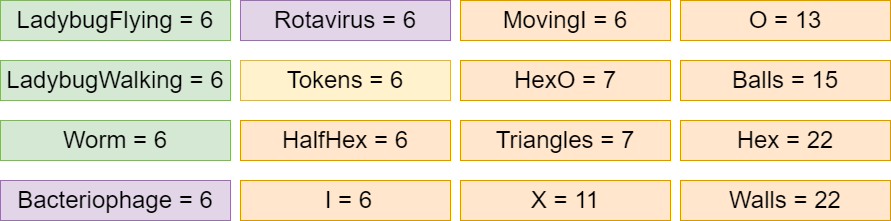
\includegraphics[width=\textwidth]{rot_values}
    \caption{\texttt{rots} values used for each obstacle type}
    \label{fig:rot_values}
\end{figure}

After addressing the the issue of game not being playable, the most straightforward method for identifying the number of rotations required was to play the game manually in debug mode. The results obtained from these experiments are displayed in Figure \ref{fig:rot_values} and were used in all experiments conducted. However, for obstacles such as \texttt{Walls} and \texttt{Balls}, this method was not viable. The reason being that running \texttt{env=Balls} or \texttt{env=Walls} with visuals caused the game to lag significantly due to the number of animations playing simultaneously. As a result, \texttt{Walls} received the same number of rotations as \texttt{Hex} trap, while \texttt{Balls} received 15 rotations, the number at which the agent managed to learn. For bug, virus, and token obstacles, the default and minimum value of 6 rotations was assigned, with which they all trained successfully.
Concerning the \texttt{dists} parameter, it was concluded during the experiments that all agents could learn any obstacle with \texttt{dists=1}, and increasing this number needlessly would only increase the number of states required for training. 

The remaining values to be determined for the experiments were the suboptions for each agent (see \ref{opt:agent}).  The reader must realize that there were a lot of experiments conducted that had to be disregarded later on for this or that reason, but they provided useful insights that could be utilized. For instance, in many of those experiments, the agent performed best with \texttt{eps} values ranging from 0.2 to 0.4, with 0.2 being the most common, in combination with an \texttt{epsFinal} value of 0.0001. The rationale for using a low \texttt{epsFinal} value is that towards the end, the agent almost exclusively exploits the current policy, and a more gradual decrease in epsilon values is suitable for larger values of \texttt{n}. Furthermore, \texttt{initOptVal} of 20.0 and 100.0 was promising in most experiments. The \texttt{gam} value will be discussed in a later subsection.

Throughout the months dedicated to conducting experiments, they gradually converged towards checking combinations of the values mentioned above. In some instances, other values were experimented with and will be discussed when exploring various environments in later subsections. However, due to the length of the experiments and the number of parameters requiring adjustment, they were kept systematic towards the end, and most of the results presented in this chapter were obtained from experiments run with different \texttt{env} and value \texttt{n} adjusted according to the environment. Each combination was tested on ten seeds for each agent, with the combinations consisting of \texttt{eps} parameter taking a value of either 0.2 or 0.4, and the \texttt{initOptVal} being either 20.0 or 100.0. Discounting was kept at the value of 1 and \texttt{epsFinal} was 0.0001.

\section{Plotting}

\begin{figure}[h]
    \centering
    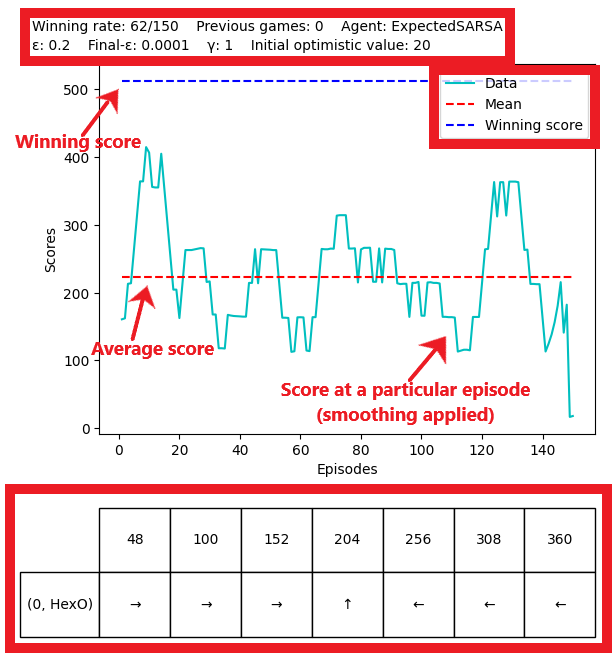
\includegraphics[width=\textwidth]{examplePlot}
    \caption{Plot example}
    \label{fig:plt_eg}
\end{figure}

In this chapter, a lot of plots similar to the one shown in Figure \ref{fig:plt_eg} will be presented. A subsection has been dedicated to explaining the different components of these plots and how to read them. While some plots may differ slightly from the one in Figure \ref{fig:plt_eg}, the meaning behind them can still be easily deduced.

The top part of the figure displays all the necessary information that was used in the experiment. Most of the values have been previously described, except for ``previous game''. This value is meant for experiments that used the \texttt{database=read} option and were performed on an agent that had trained for some number of games. This number specifies the how many of games the agent had previously trained on.

Moving further down, there is a plot with three lines and a legend in the top right corner. The data line, as indicated on the figure, represents the score that the agent achieved on a particular episode. However, some plots may show the average value of the agent's score for that episode over several different seeds used for the random action. Additionally, there may be multiple data lines on the plot, each representing a different agent. In these cases, each line is averaged between many seeds. Each agent is labelled with their respective color inside the legend.

The mean line represents the average score value for the entire experiment, while the winning score represents the winning threshold. It should be noted that if the agent did not win any games, the winning score line will be omitted. Furthermore, the data line is averaged to appear smoother. This is why even though the winning rate is 62/150, the data line doesn't touch the winning score threshold at any point.

As mentioned in the Section \ref{commOpt}, it is possible to perform continuous evaluation on experiments, meaning one learning game is played with random actions, followed immediately by an evaluation game using only the current policy that the agent is performing. In all experiments conducted, the data line only represents the evaluation games.

At the very bottom of the figure, there is a table which only appears in plots that contain a single data line that is not averaged over different seeds and has only one seed value. In the table, all rotation values for this experiment define the columns, while each row has a tuple of distance value and type of the obstacle. Since all experiments are performed on \texttt{dists=1}, the number of rows will match only the number of different obstacles used in the experiment.

It should be emphasized that parameters such as the number of seeds in the averaged data line or the size of the smoothing window will be clearly specified for each plot mentioned in the rest of the chapter. This prevents any form of ambiguity or confusion regarding the details of the experiment.

\section{Interesting behaviours}
\label{intbeh}
\begin{figure}[h]
    \centering
    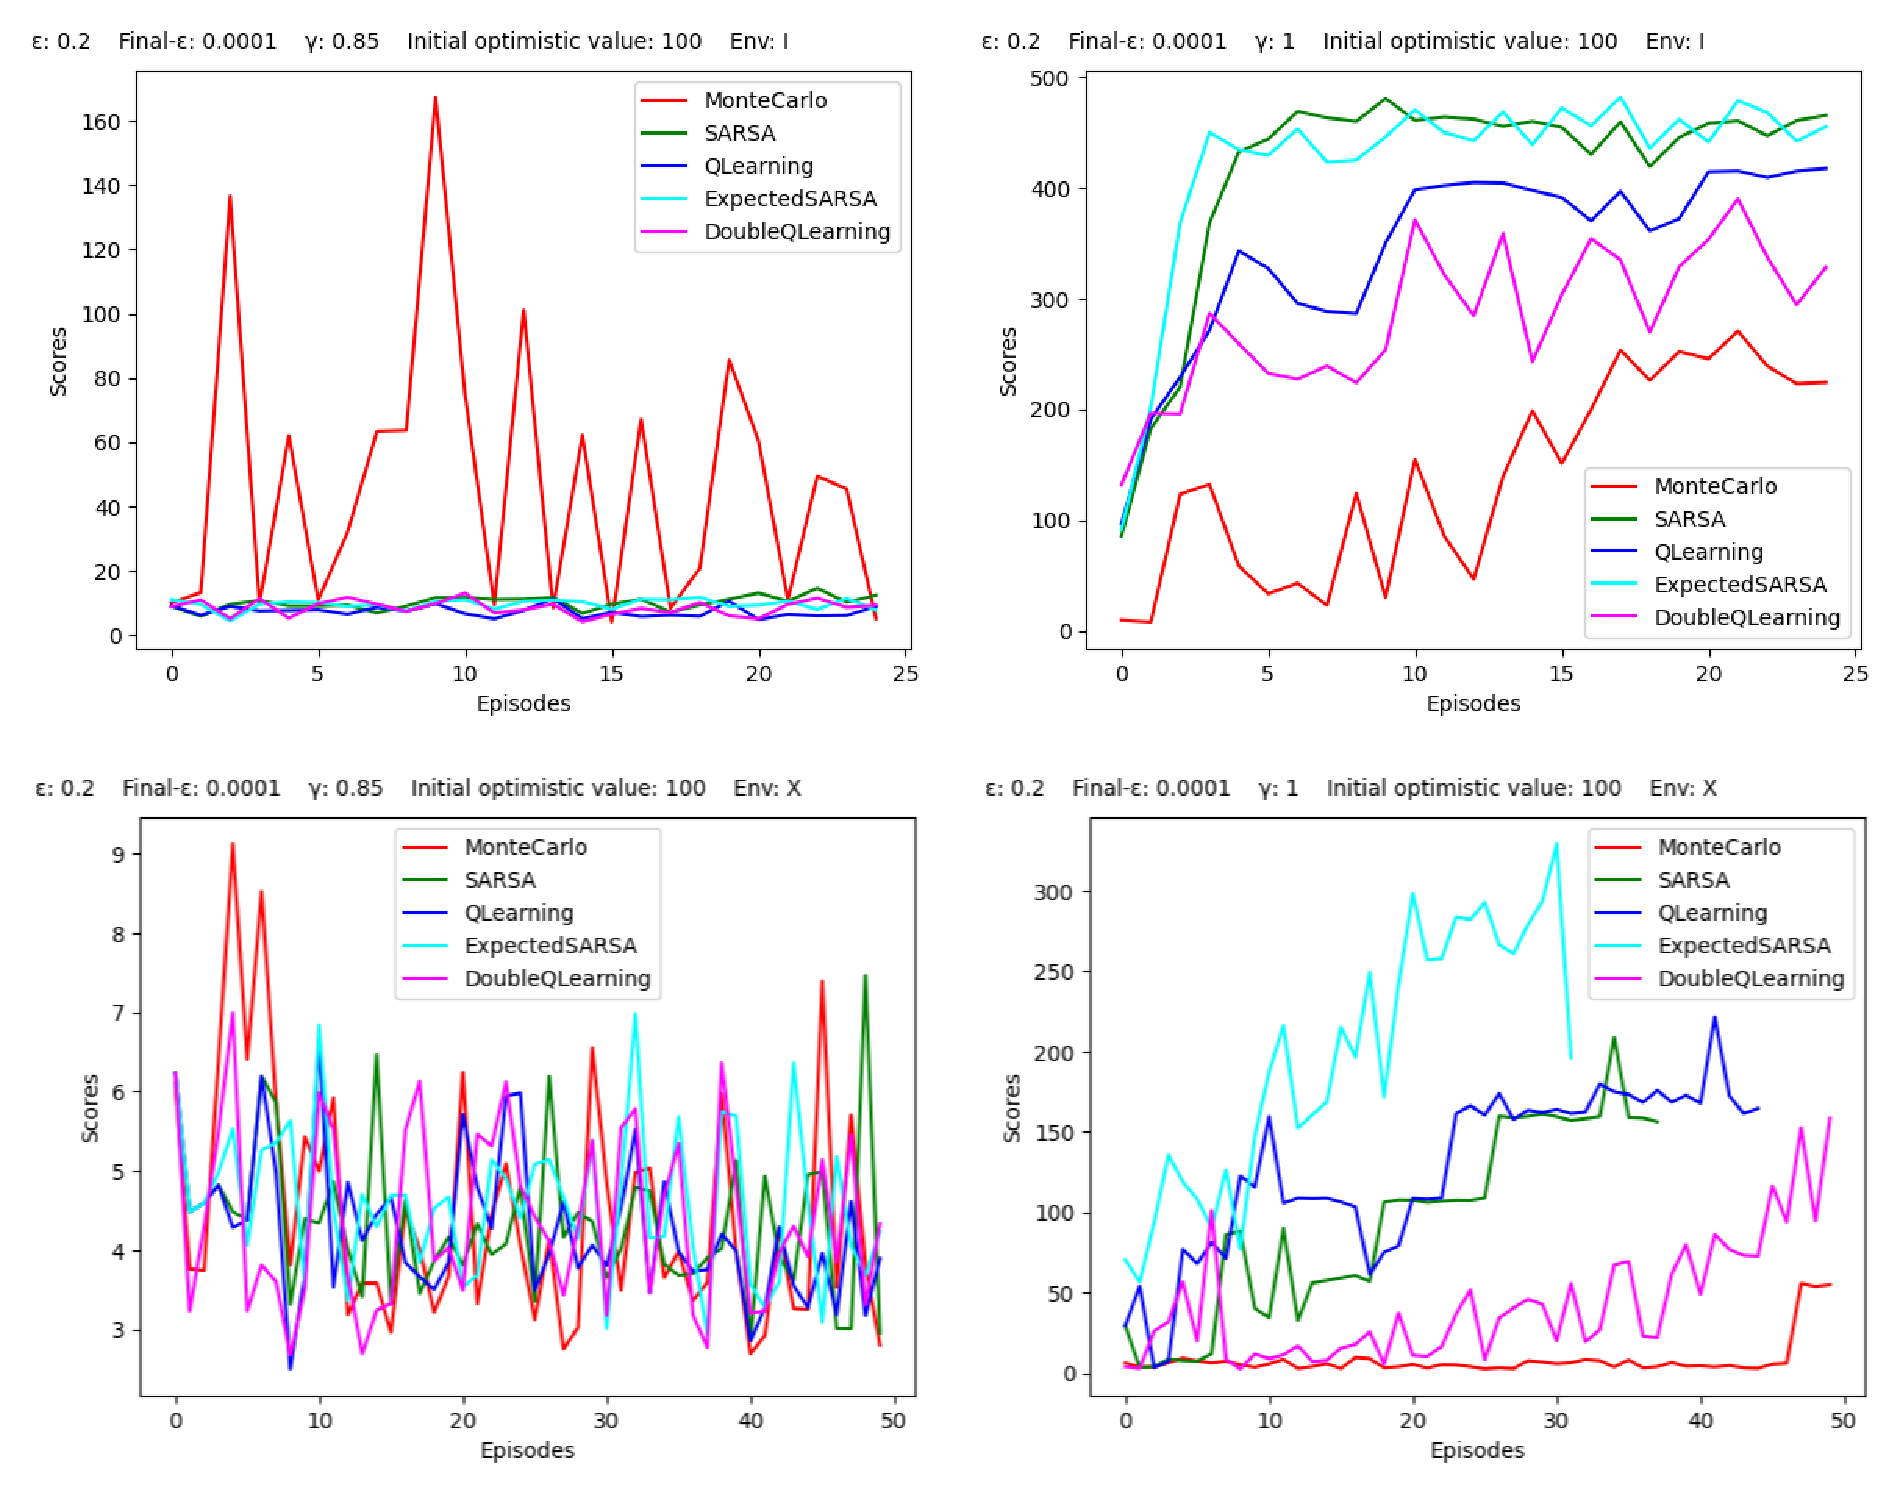
\includegraphics[width=\textwidth]{discountingExample}
    \caption{Discounting example}
    \label{fig:discounting_eg}
\end{figure}

In this chapter, we aim to discuss certain unexpected findings that surfaced during our experimentation. One of the immediate observations can be seen in Figure \ref{fig:discounting_eg}\footnote{No smoothing was applied to any of the plots in this subsection}. We conducted experiments on two distinct environments, \texttt{env=[I]} and \texttt{env=[X]}, and for each environment, we carried out experiments with \\ \texttt{gam=0.85} and \texttt{gam=1.0} for all agents. As evident from the plots, the lower gamma value exhibited considerably poorer performance than when no discounting (\texttt{gam=1.0}) was applied. This trend is not limited to these specific environments and testing conditions but rather observed consistently across all our experimentation. This result is counter-intuitive since it seems logical that penalizing the last action more than previous ones would result in a better policy.

\label{intbeh}
\begin{figure}[h]
    \centering
    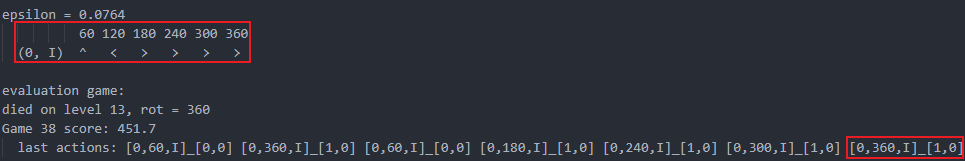
\includegraphics[width=\textwidth]{discountingExplanation}
    \caption{Discounting explanation}
    \label{fig:discounting_expl}
\end{figure}

Upon further investigation, we discovered that in some cases, a lost game for the agent does not result from the last action directly but rather from a chain reaction initiated by a previous ``bad decision''. As seen in Figure \ref{fig:discounting_expl}, the agent's last action of going right at rotation \texttt{360} to reach a safe one, \texttt{60}, is not a poor decision in itself but rather the best possible action in that state\footnote{As confirmed by a human player, rotation 60 is safe for trap type I}. However, analysing the last four actions taken by the agent, it becomes clear that it attempted to reach rotation \texttt{60} by going left from the rotation \texttt{180}. With a high score of \texttt{451.7} (Figure \ref{fig:discounting_eg}), the agent was undeniably fast, and while this policy may have been effective in the early game before the agent attained its current speed\footnote{It should recalled that after every 3 levels the agents speed increases}, there is simply not enough time for the agent to rotate at this point in the game. In this case, one could argue that the fourth action from the last was responsible for the agent's loss. For cases like this, we believe that the agent performs better when all actions are penalized equally.


\label{intbeh}
\begin{figure}[h]
    \centering
    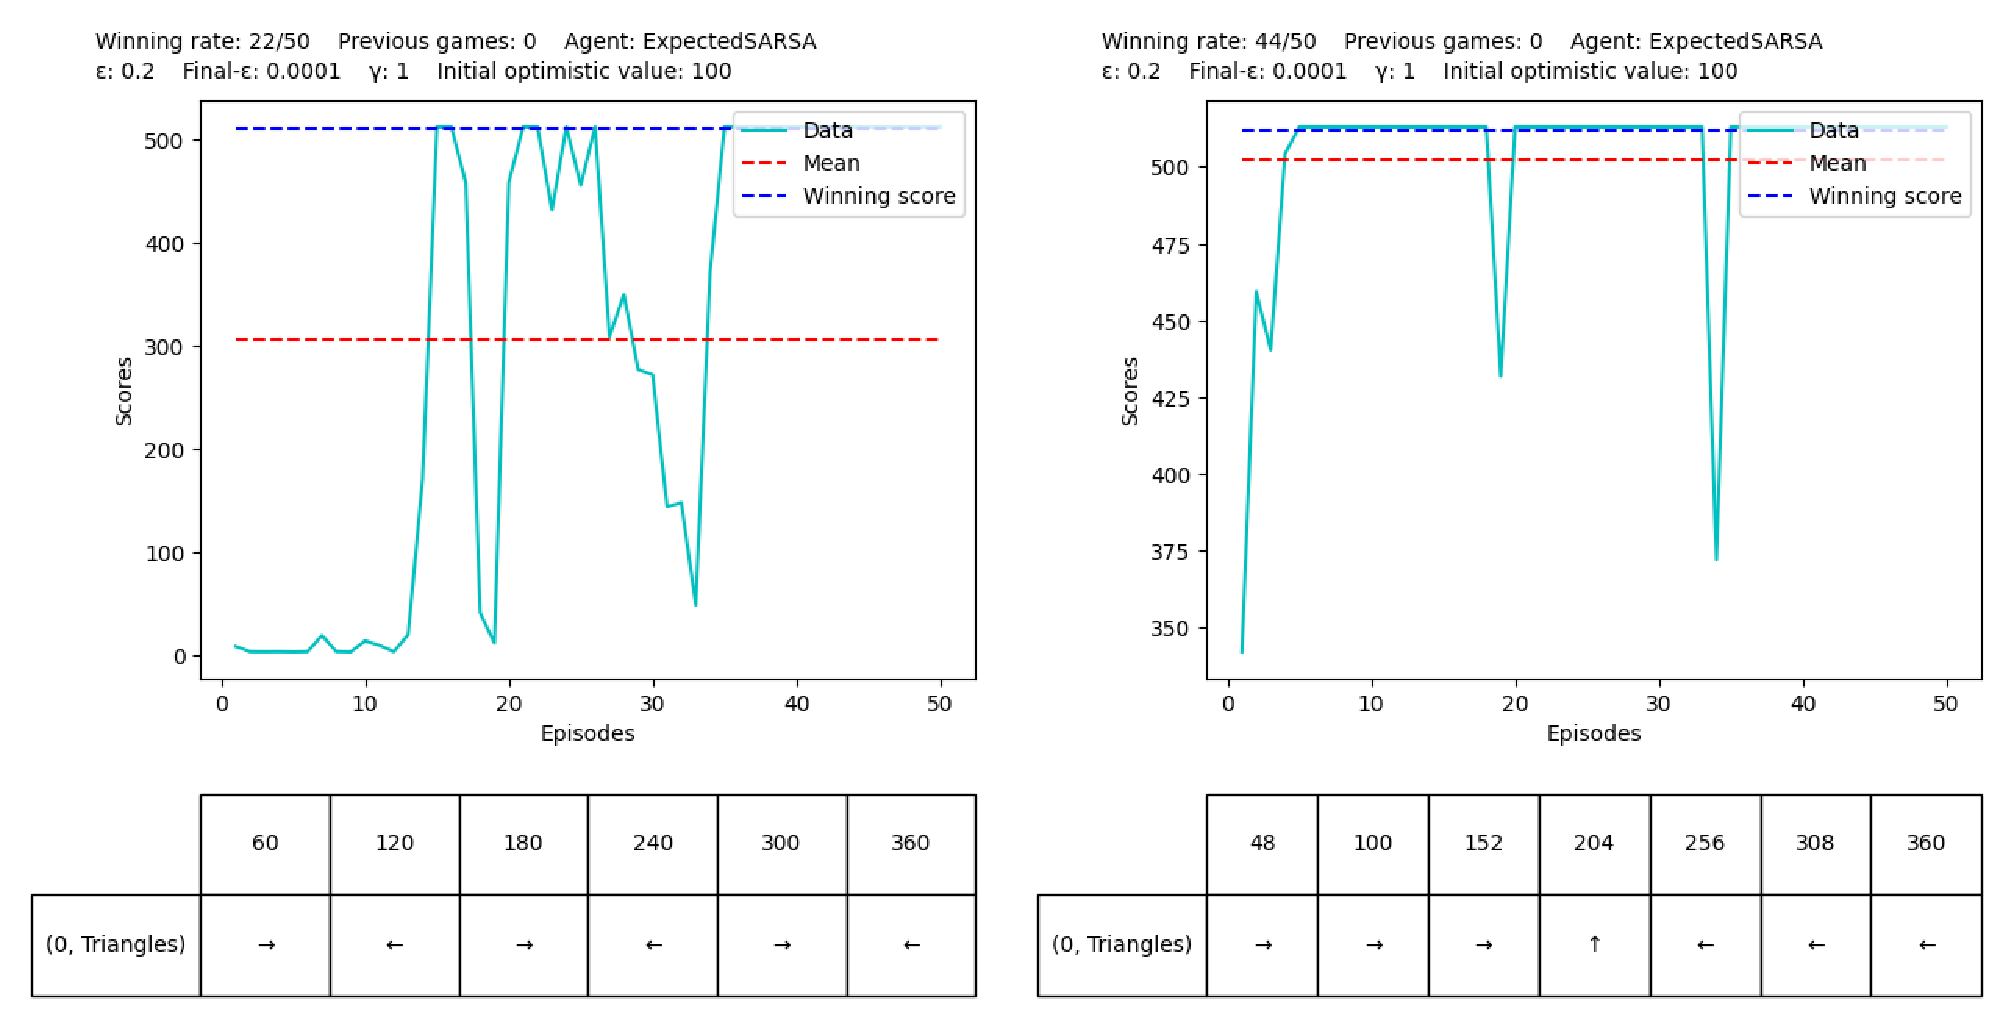
\includegraphics[width=\textwidth]{trianglesExample}
    \caption{Triangles example}
    \label{fig:triangles_eg}
\end{figure}

Another intriguing behaviour emerged as a result of an unforeseen coincidence. As previously noted, we chose to have the agent not take a new action every time its \texttt{move()} function is called, but rather return the same action until the state changes. This resulted in a substantial reduction in the number of different actions taken by the agent, given that the move function is invoked every game tick, while state changes occur less frequently. This approach led to a behaviour that could not have been predicted at the outset. Figure \ref{fig:triangles_eg} provides an illustration of this behaviour (with some sentiment \texttt{env=[Triangles]} was chosen as this was the first environment on which the behaviour was noticed).

Ordinarily, \texttt{env=[Triangles]} does not offer any safe rotations unless \texttt{rots=7} or more. As shown in the plot, the agent will certainly learn with this rotation value. However, if the agent is given only \texttt{6} rotation values to choose from, it will develop a policy that rapidly oscillates between two rotations, keeping the player character, Hans, on the edge of those rotations, allowing him to safely pass through the trap. This behaviour is not confined to situations where the agent is ``forced'' to make such a decision. During training, in many instances, the agent will learn to stay on the edge rather than advance into a completely safe rotation. There does not appear to be a preference for one or the other; rather, the policy the agent discovers first is determined by other experimental factors. It can be concluded that this behaviour arose solely because the agent did not alter its action until the state changed. In my opinion, this discovery is one of the most exciting outcomes of this project.

\section{Individual traps environment}
\section{Traps environment}
\section{Tokens environment}
\section{Bugs environment}
\section{Viruses environment}
\section{Full game environment}